\documentclass[tikz,border=9pt]{standalone}
\usepackage{amsmath,amssymb}
\usetikzlibrary{arrows.meta,positioning,calc}
\begin{document}
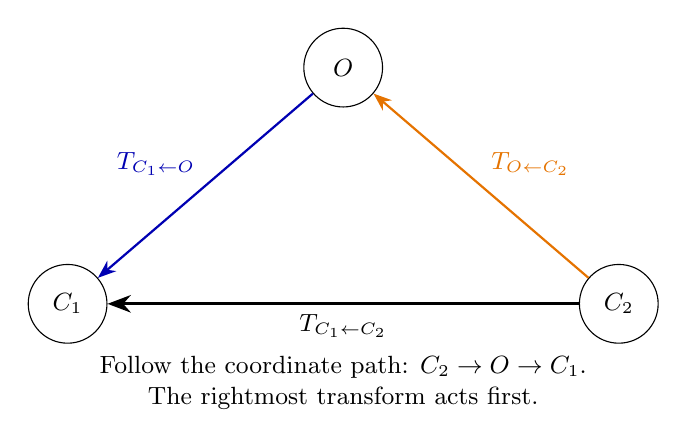
\begin{tikzpicture}[font=\small,arr/.style={-{Stealth},thick},box/.style={draw=blue!55!black,rounded corners,fill=blue!4,align=center,text width=2.9cm,minimum height=1.05cm}]

\node[draw,circle,minimum size=1cm] (a) at (0,0) {$C_1$};
\node[draw,circle,minimum size=1cm] (b) at (7,0) {$C_2$};
\node[draw,circle,minimum size=1cm] (o) at (3.5,3) {$O$};
\draw[arr,blue!70!black] (o)--(a) node[midway,above left]{$T_{C_1\leftarrow O}$};
\draw[arr,orange!90!black] (b)--(o) node[midway,above right]{$T_{O\leftarrow C_2}$};
\draw[arr,very thick] (b)--(a) node[midway,below]{$T_{C_1\leftarrow C_2}$};
\node[align=center] at (3.5,-1){Follow the coordinate path: $C_2\to O\to C_1$.\\The rightmost transform acts first.};

\end{tikzpicture}
\end{document}
